
\section{Results}
\label{sec:results}

% Present the results of your experiments. Simply presenting the data is
% insufficient! You need to analyze your results. What did you discover?
% What is interesting about your results? Were the results what you
% expected? Use appropriate visualizations. Prefer graphs and charts to
% tables as they are easier to read (though tables are often more
% compact, and can be a better choice if you're squeezed for space).


\subsection{Results of Experiment 1: Parameter Settings}
\label{sec:resE1}
Since we had a limited number of future states in each game, the first and last states in a game were close to each other. Thus, changes in gamma minimally impacted the performance of the Q-learning bot. Since our algorithm was not particularly expensive in terms of either space or time complexity, we were able to train our policy on a large number of hands. Thus, alpha had minimal impact on the performance of our algorithm because we trained the policy on 1,000,000 hands. The lack of correlation between the alpha and gamma settings with average rewards is shown in Figure \ref{hpFig}. This graph shows that these parameters had little to no effect on the average rewards of the Q-learning bot. 

\begin{figure}[htb]

  \centering  % centers the image in the column

  % replace the second argument below with your filename. I like to
  % place all my figures in a sub-directory to keep things organized
  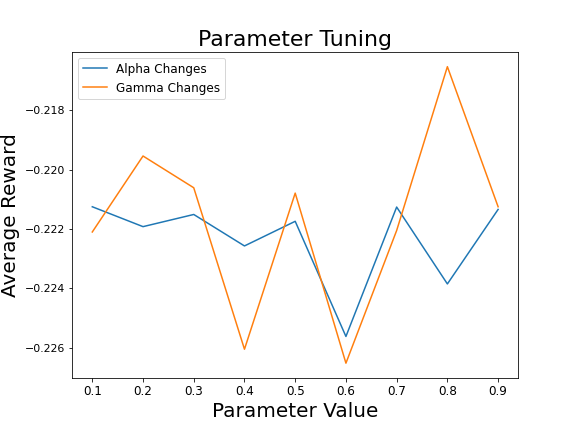
\includegraphics[width=0.47\textwidth]{hpTuning.png}


  % *Every* figure should have a descriptive caption.
  \caption{Comparison of average rewards for policies trained with varying alpha and gamma values.}

  \label{hpFig}

\end{figure}

\subsection{Results of Experiment 2: Player Performance}
\label{sec:resE2}
As shown in Figure \ref{avgRewards}, our bot quickly outperformed the random player, reaching higher average rewards after only a few thousand hands. Subsequently, our bot failed to improve its performance, however. Figure \ref{avgRewards} shows the Q-learning bot's early plateau: failing to improve at all after about 20,000 hands. In our experiment, the Q-learning bot failed to converge to an optimal policy or anything remotely close to optimal. Our bot averaged a reward of $-22$ percent whereas an optimal policy should make returns close to $-4$ percent. The random bot realized approximately $-25$ percent returns, just 3 percentage points worse than our player. These results suggest that our Q-learning bot was not able to effectively learn optimal policies that mirrored those used in the heuristic bot.\\

\noindent Furthermore, the assumption that the dealer's hidden card is of value 10 proved to have no impact on the performance of our player. We experimented with and without the assumption on different parameter settings, but the Q-learning bot realized average returns which were 99 percent similar, both converging to approximately $-22$ percent. 

\begin{figure}[htb]

  \centering  % centers the image in the column

  % replace the second argument below with your filename. I like to
  % place all my figures in a sub-directory to keep things organized
  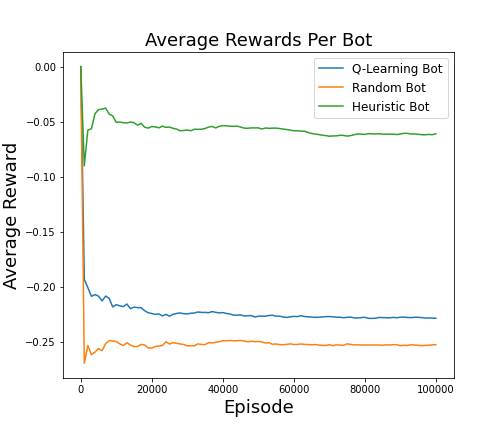
\includegraphics[width=0.47\textwidth]{avgRewardsPerBot.png}


  % *Every* figure should have a descriptive caption.
  \caption{Comparison of average rewards for the Q-learning bot, random bot, and heuristic bot.}

  \label{avgRewards}

\end{figure}



